%%
%% Dit is de domeinanalyse: Combinatorial Objects
%%
\documentclass[a4paper,11pt,final]{article}

\usepackage{subfig}
\usepackage{wrapfig}% product wrapfigure and wraptable
\usepackage{array}% additions to tabular
\usepackage{supertabular}% multiple pages tabular
\usepackage{rotating}% for the environment sidewaysfigure / sidewaystable
\usepackage[english]{babel}
\usepackage{graphicx}
\usepackage{hyperref}
\hypersetup{
    colorlinks = true,
    citecolor = blue,
    linkcolor = blue
}
\usepackage[prependcaption,colorinlistoftodos,obeyFinal,textsize=tiny]{todonotes}% when generating final (documentclass option) skip notes
\usepackage{pdflscape}
\usepackage[a4paper]{geometry}
\usepackage{titlesec}% added to change section headers, see newcommand definition.
\usepackage{boxedminipage}
\usepackage{amssymb}% For \checkmark
\usepackage{pifont}% for \ding{'-code or "-code}

\bibliographystyle{alpha}

		

\begin{document}
\selectlanguage{english}

\begin{titlepage}
	\vspace*{\fill}
    \begin{center}
    	\textsc{\large WickedXmas Domain Analysis}\\[0.5cm]
    	\textsc{\huge Combinatorial Objects}\\[0.5cm]
		\textsc{Stefan Versluys}\\
		\textsc{\scriptsize 19/10/2014}\\[2.0cm]
		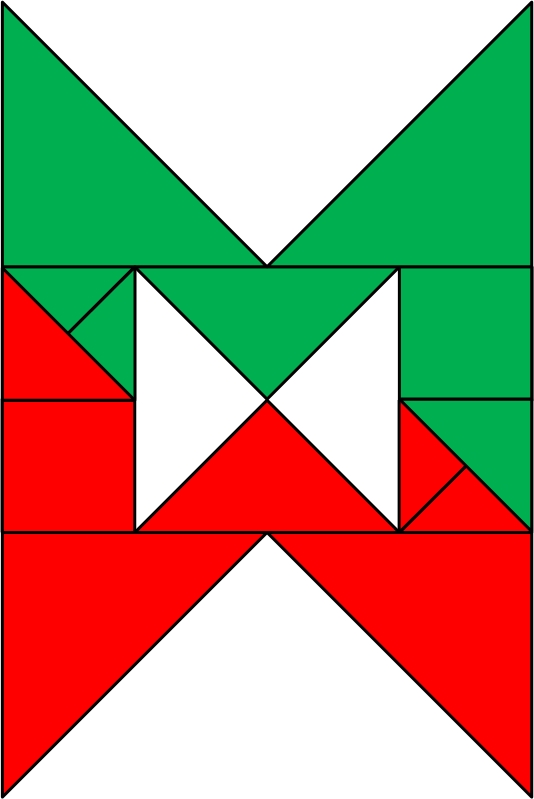
\includegraphics[width=0.25\textwidth]{wXm}
	\end{center}
	\vspace*{\fill}
\end{titlepage}


\tableofcontents
\newpage


\section{Introduction}
This domain analysis concerns combinatorial objects, along with primitive objects this kind of objects can be used to design xMAS models with the WickedXmas tool. In fact combinatorial objects are xMAS models itself but left open with unconnected ports, parameterizable and allow recursive reuse.\\
The benefits of combinatorial objects are those of re-usability, it makes complex things look simple and maintainable, it preserves correctness.\\
When designing an xMAS model in WickedXmas , the designer can make use of combinatorial objects similar as he or she does with primitive objects. Because combinatorial objects are xMAS models these can be edited just as any other kind of xMAS model except that there are unconnected ports as mentioned before.

\section{Dictionary} 
Before we can continue explaining this matter, we need a vocabulary. 
\begin{itemize}
\item \textbf{WickedXmas}: Name of the tool used to design and analyse xMAS models.
\item \textbf{xMAS model}: A model based on Intel's xMAS or e\underline{x}ecutable \underline{M}icro\underline{A}rchitectural \underline{S}pecification, which is a high level design language for communication fabrics. 
\item \textbf{Primitive Object}: The xMAS language consist of eight primitive objects which are used to create xMAS models. Primitive objects are hard coded.
\item \textbf{Combinatorial Object}: A composite object which can be made of primitives and combinatorial objects. It is also known as a open xMAS model or macro.
\item \textbf{Channel}: A connection between an input and output port.
\item \textbf{Port}: Each object has one or more ports to create a channel, there are initiator and target ports.
\item \textbf{Initiator}: An output port.
\item \textbf{Target}: An input port.
\item \textbf{Open xMAS network}: see combinatorial object.
\item \textbf{Macro}: see combinatorial object.


\end{itemize}


\newpage
\section{Primitive objects}
Primitive objects are the base of combinatorial objects and determine the underlying structures. Secondly, when using objects to create a model, there are a lot of similarities between combinatorial and primitive objects. With this knowledge we can say that primitive objects need some explanation as far as these are concerned with combinatorial objects.
\\The xMAS language has only eight primitive objects, each object has a visual representation and one or more properties which can be changed by the user. Some of these properties requires a valid value otherwise a visual marker, shown as a dot as part of the object, will lit up red instead of green. Finally all objects have one or more ports, ports can be of target or input type and initiator or output type, ports are represented by red filled squares. All ports must be wired to an opposite type of port of a other object to form a valid channel.


% wich will be discribed in the next subsections. 
\subsection{Queue}
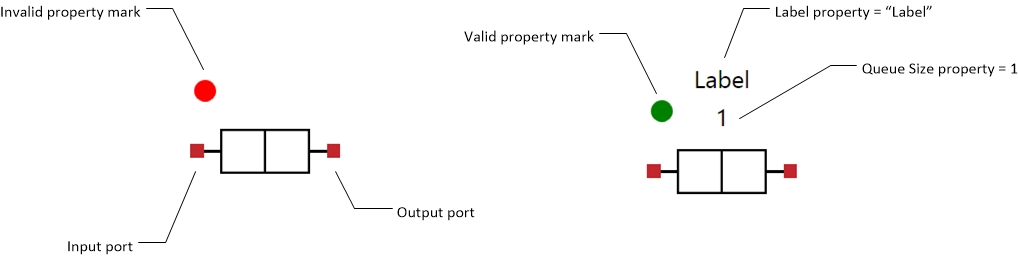
\includegraphics[width=0.5\textwidth]{queue}
ToDo : description + fjson structure
\subsection{Function}
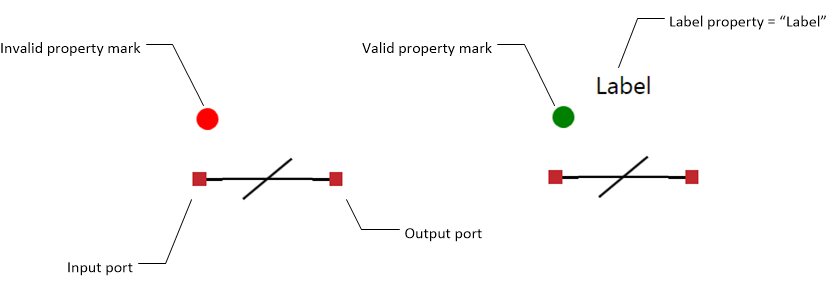
\includegraphics[width=0.5\textwidth]{function}
\\Property "Function f" is a subset of the C language, an integer which represents the packet is available through variable 'header'. 
\begin{itemize}
\item math operators $+,-,*,/,\%$
\item logical operators $\&\&,||,!$
\item equality operators $==,<=,>=,<,>$
\end{itemize} 
Example function : ret=0;
\\ToDo : description + fjson structure
\subsection{Fork}
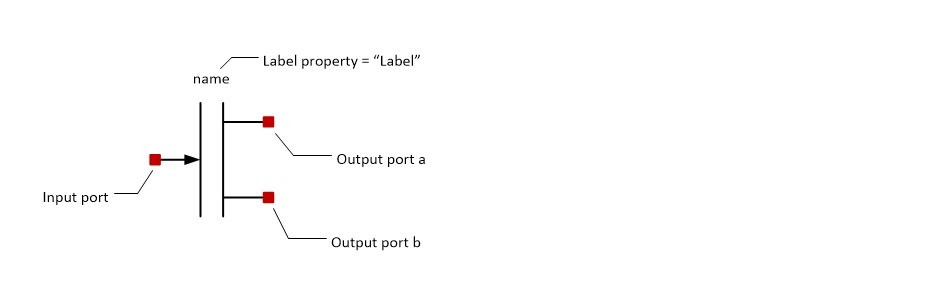
\includegraphics[width=0.25\textwidth]{fork}
\\ToDo : description + fjson structure
\subsection{Join}
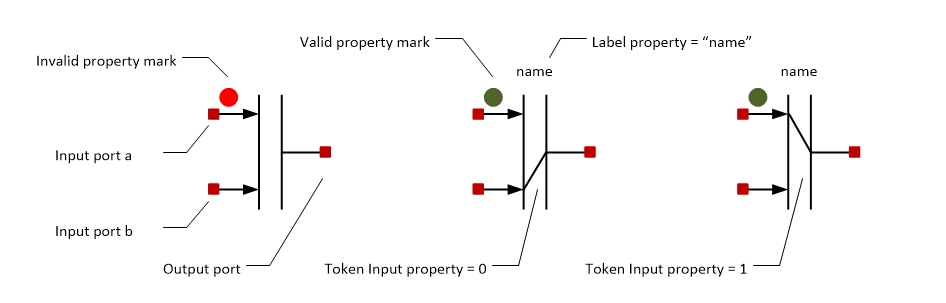
\includegraphics[width=0.5\textwidth]{join}
\\ToDo : description + fjson structure
\subsection{Switch}
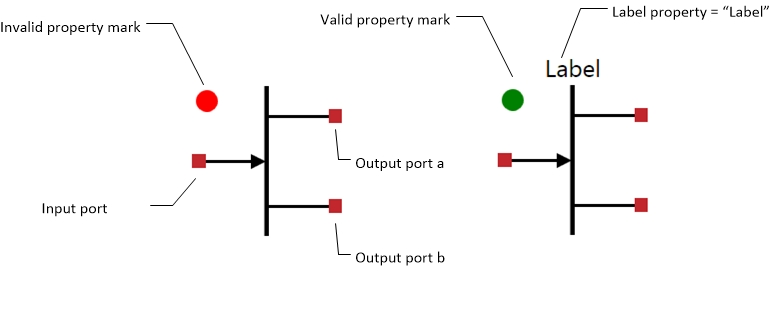
\includegraphics[width=0.5\textwidth]{switch}
\\Property "Function s" is a subset of the C language, an integer which represents the packet is available through variable 'header'. 
\begin{itemize}
\item math operators $+,-,*,/,\%$
\item logical operators $\&\&,||,!$
\item equality operators $==,<=,>=,<,>$
\end{itemize} 
Example function : return header == 0;
\\ToDo : description + fjson structure  
\subsection{Merge}
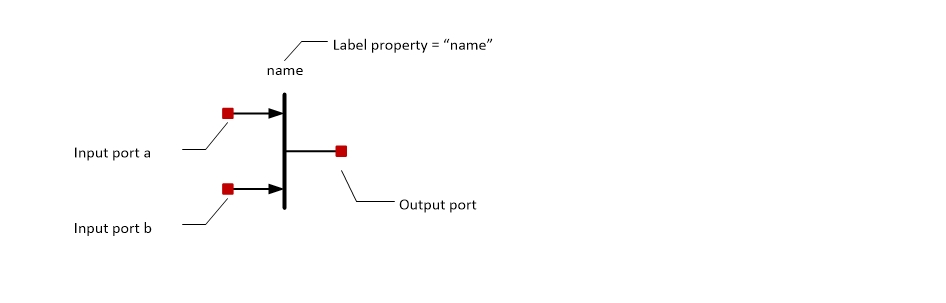
\includegraphics[width=0.3\textwidth]{merge}
\\ToDo : description + fjson structure
\subsection{Sink}
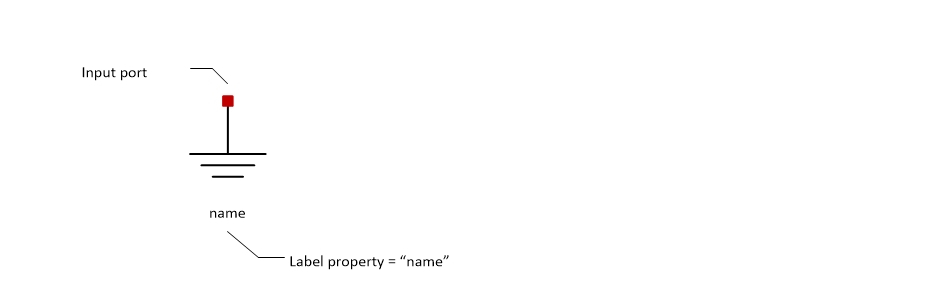
\includegraphics[width=0.5\textwidth]{sink}
\\ToDo : description + fjson structure
\subsection{Source}
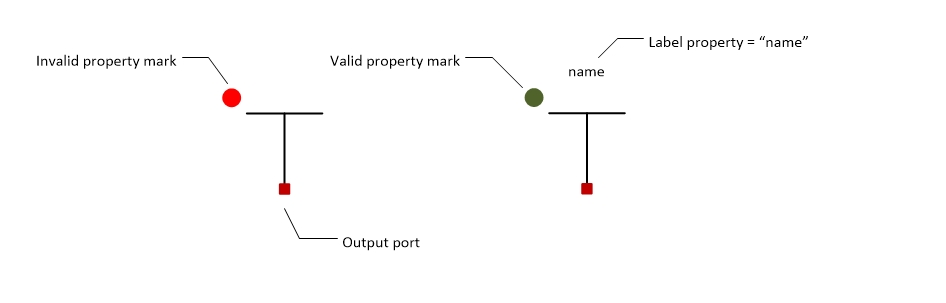
\includegraphics[width=0.5\textwidth]{source}
\\Property "Function e" insert types of packets injected at this source. The domain of all packets is available through PacketDomain. 
\\ToDo : description + fjson structure

\newpage
\section{Combinatorial objects}
To create combinatorial objects, which means an open network, we need something to distinguish between an dangling port or a port that can be connected later when re-using the combinatorial object. Example : {p in PacketDomain | p < 100}
\\ToDo : to be completed
\subsection{Recursion}
\subsection{Macro}
\subsection{Visual representation}
\subsection{Structure}

\newpage
\section{Structures}
ToDo : to be completed
\subsection{Hierarchical structure}
\subsection{Flat structure}

\newpage
\section{Similar domain examples}
ToDo : example of how a similar product manages re-usable components 



\end{document} ;########################### end document ##################################;